% !TeX spellcheck = en_GB
% !TeX root = ../phd-thesis.tex

\begin{figure*}
    \centering
    \caption{
        Example of the encoding process of logic formulas into real-values functions.
        %
        Only \gls{AST} are depicted. Box coloured in the same way represent the encoding of a given operator through each encoding step.
        %
        So, for instance, operator $<$ (red) is firstly converted into a negated $\geq$, and then in a combination of $max$ and subtractions.
    }
    \begin{subfigure}[]{0.3\linewidth}
        \centering
        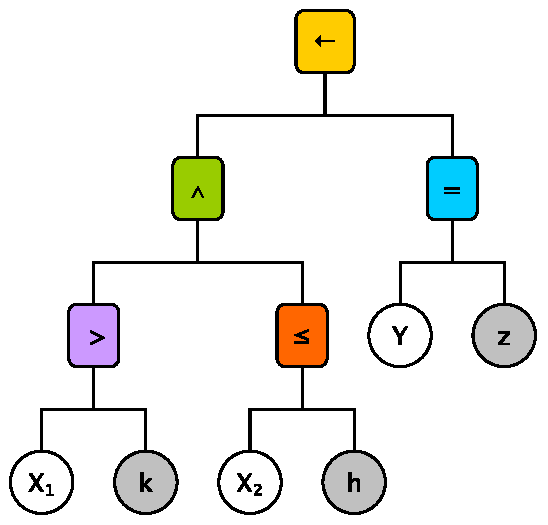
\includegraphics[scale=\astscale]{figures/ast-unencoded}
        \caption{AST of a logic formula}
        \label{fig:ast-unencoded}
    \end{subfigure}
    $\rightarrow$
    \begin{subfigure}[]{0.3\linewidth}
        \centering
        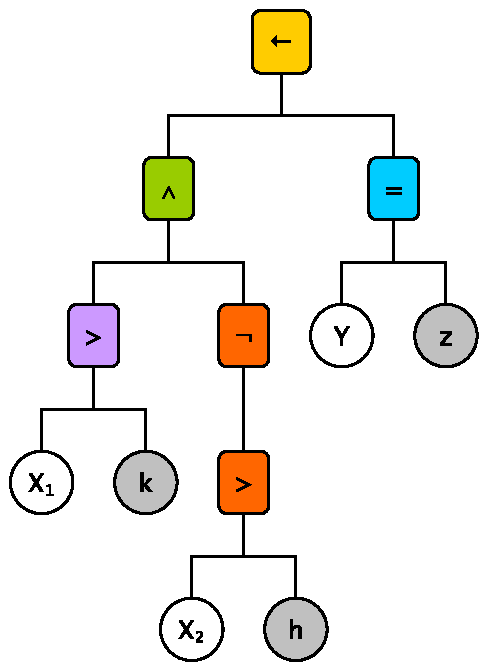
\includegraphics[scale=\astscale]{figures/ast-simplified}
        \caption{Simplified AST of a logic formula}
        \label{fig:ast-simplified}
    \end{subfigure}
    $\rightarrow$
    \begin{subfigure}[]{0.3\linewidth}
        \centering
        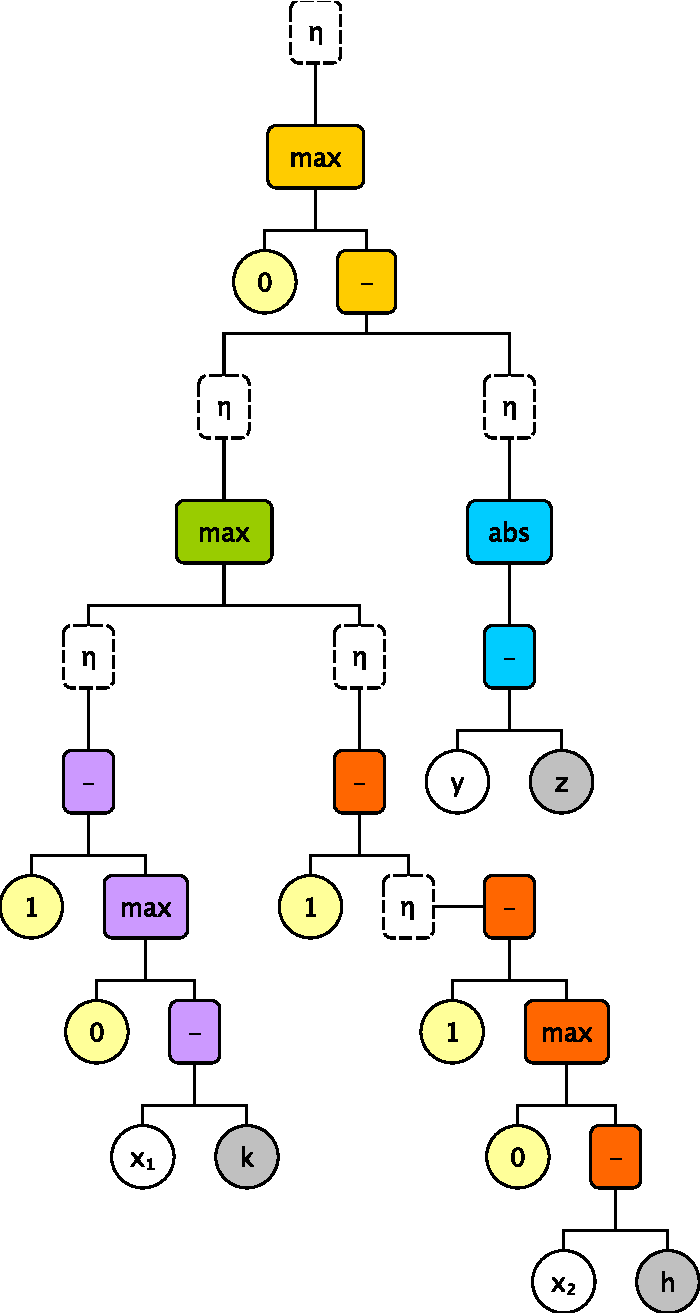
\includegraphics[scale=\astscale]{figures/ast-encoded}
        \caption{AST of the same formula, encoded as real-valued function}
        \label{fig:ast-encoded}
    \end{subfigure}
    \label{fig:ast}
\end{figure*}
